\section{Appendix: Graphs and Visualizations}

% Logistic Regression: Training and Validation Loss (Grouped by Learning Rate)
\subsection{Logistic Regression: Training and Validation Loss}
\begin{figure}[htbp!]
    \centering
    \begin{subfigure}{0.32\textwidth}
        \centering
        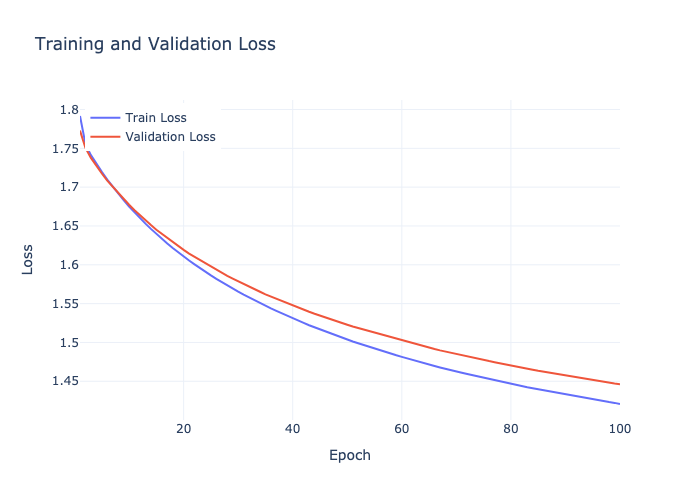
\includegraphics[width=\textwidth]{images/logistic_regression-training-validation-loss-batch-32-lr-1e-05-epochs-100-l2-0.01-opt-sgd.png}
        \caption{LR = $10^{-5}$}
    \end{subfigure}
    \begin{subfigure}{0.32\textwidth}
        \centering
        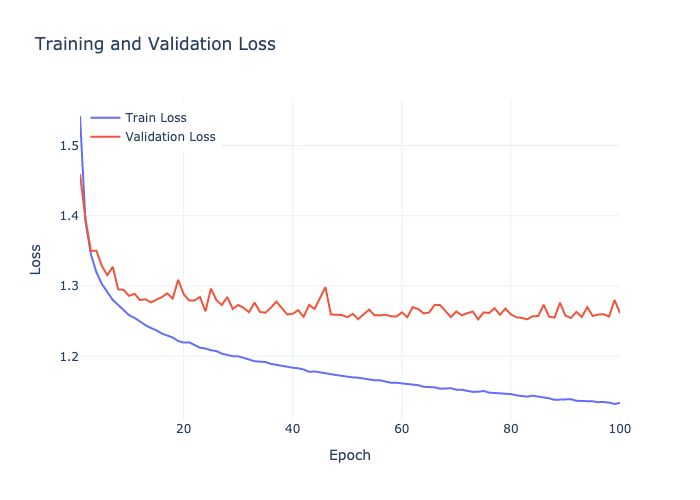
\includegraphics[width=\textwidth]{images/logistic_regression-training-validation-loss-batch-32-lr-0.001-epochs-100-l2-0.01-opt-sgd.png}
        \caption{LR = $10^{-3}$}
    \end{subfigure}
    \begin{subfigure}{0.32\textwidth}
        \centering
        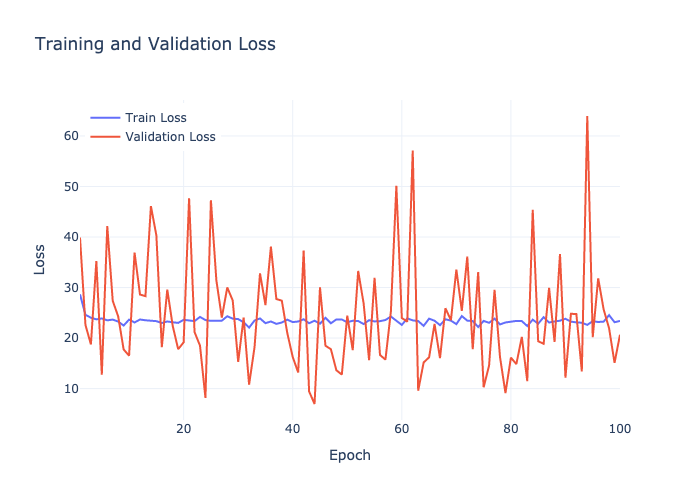
\includegraphics[width=\textwidth]{images/logistic_regression-training-validation-loss-batch-32-lr-0.1-epochs-100-l2-0.01-opt-sgd.png}
        \caption{LR = $0.1$}
    \end{subfigure}
    \caption{Logistic Regression: Training and Validation Loss for different Learning Rates.}
    \label{fig:log_reg_loss}
\end{figure}

% Logistic Regression: Validation Accuracy (Grouped by Learning Rate)
\subsection{Logistic Regression: Validation Accuracy}
\begin{figure}[htbp!]
    \centering
    \begin{subfigure}{0.32\textwidth}
        \centering
        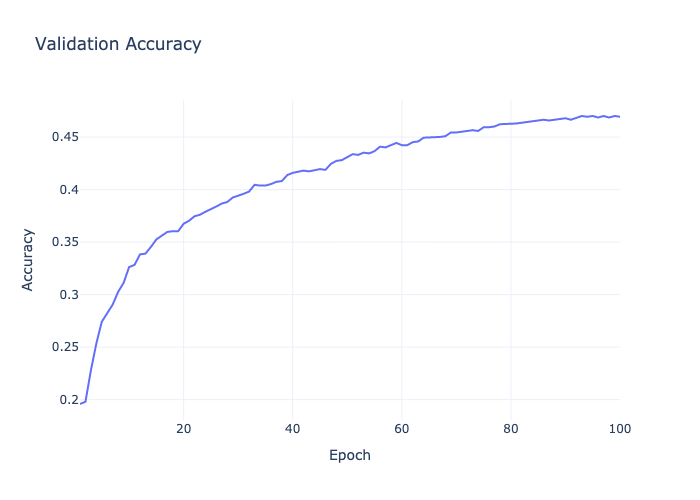
\includegraphics[width=\textwidth]{images/logistic_regression-validation-accuracy-batch-32-lr-1e-05-epochs-100-l2-0.01-opt-sgd.png}
        \caption{LR = $10^{-5}$}
    \end{subfigure}
    \begin{subfigure}{0.32\textwidth}
        \centering
        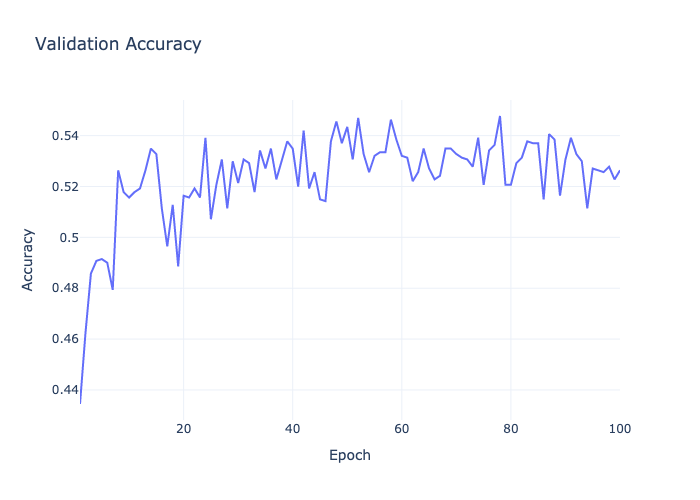
\includegraphics[width=\textwidth]{images/logistic_regression-validation-accuracy-batch-32-lr-0.001-epochs-100-l2-0.01-opt-sgd.png}
        \caption{LR = $10^{-3}$}
    \end{subfigure}
    \begin{subfigure}{0.32\textwidth}
        \centering
        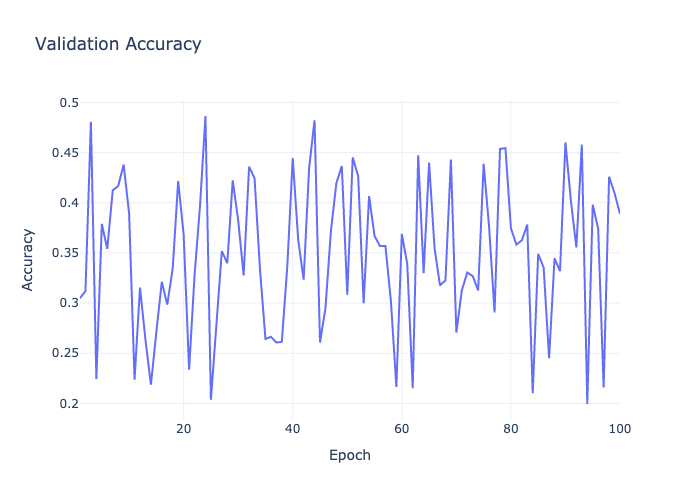
\includegraphics[width=\textwidth]{images/logistic_regression-validation-accuracy-batch-32-lr-0.1-epochs-100-l2-0.01-opt-sgd.png}
        \caption{LR = $0.1$}
    \end{subfigure}
    \caption{Logistic Regression: Validation Accuracy for different Learning Rates.}
    \label{fig:log_reg_acc}
\end{figure}


\subsubsection{Default Hyperparameters vs. Batch Size = 512}
The effect of varying the batch size between the default (64) and a larger value (512) was explored.

\begin{figure}[htbp!]
    \centering
    \begin{subfigure}{0.45\textwidth}
        \centering
        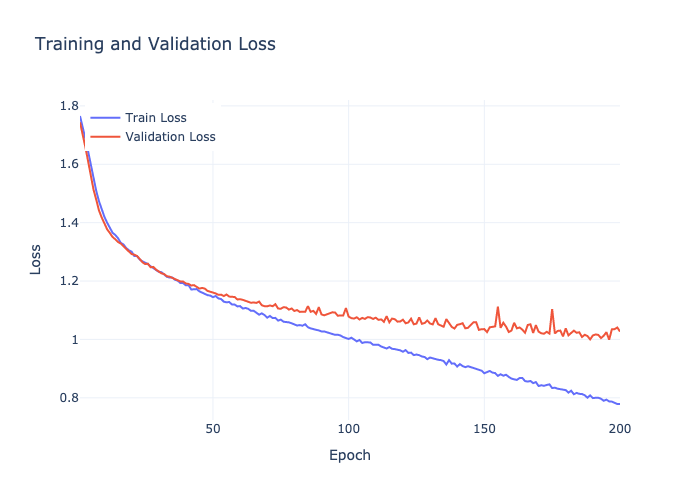
\includegraphics[width=\textwidth]{images/mlp-training-validation-loss-batch-64-lr-0.002-epochs-200-hidden-200-dropout-0.3-l2-0.0-layers-2-act-relu-opt-sgd-mom-0.0.png}
        \caption{Batch Size = 64}
    \end{subfigure}
    \hfill
    \begin{subfigure}{0.45\textwidth}
        \centering
        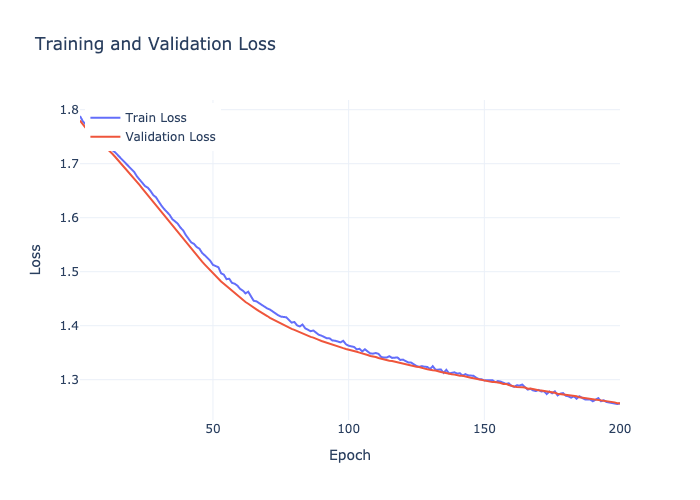
\includegraphics[width=\textwidth]{images/mlp-training-validation-loss-batch-512-lr-0.002-epochs-200-hidden-200-dropout-0.3-l2-0.0-layers-2-act-relu-opt-sgd-mom-0.0.png}
        \caption{Batch Size = 512}
    \end{subfigure}
    \caption{MLP: Training and Validation Loss for different Batch Sizes.}
    \label{fig:mlp_batch_size_loss}
\end{figure}

\clearpage

\begin{figure}[htbp!]
    \centering
    \begin{subfigure}{0.45\textwidth}
        \centering
        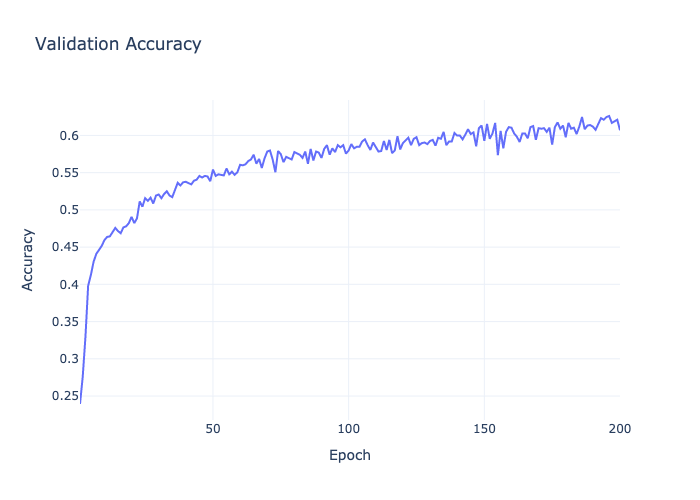
\includegraphics[width=\textwidth]{images/mlp-validation-accuracy-batch-64-lr-0.002-epochs-200-hidden-200-dropout-0.3-l2-0.0-layers-2-act-relu-opt-sgd-mom-0.0.png}
        \caption{Batch Size = 64}
    \end{subfigure}
    \hfill
    \begin{subfigure}{0.45\textwidth}
        \centering
        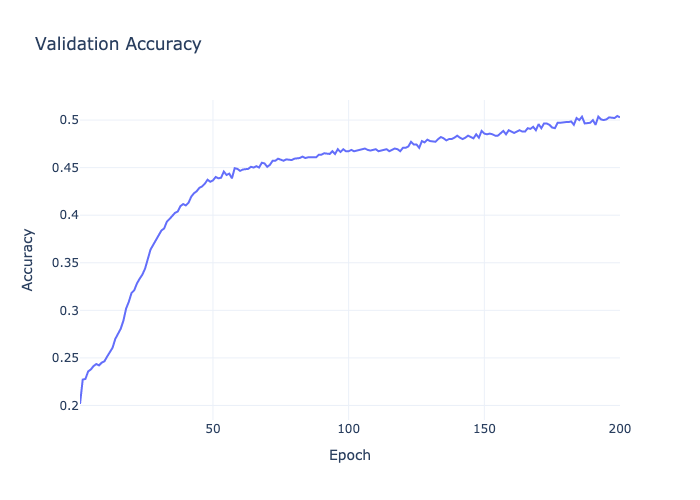
\includegraphics[width=\textwidth]{images/mlp-validation-accuracy-batch-512-lr-0.002-epochs-200-hidden-200-dropout-0.3-l2-0.0-layers-2-act-relu-opt-sgd-mom-0.0.png}
        \caption{Batch Size = 512}
    \end{subfigure}
    \caption{MLP: Validation Accuracy for different Batch Sizes.}
    \label{fig:mlp_batch_size_acc}
\end{figure}



% MLP: Training and Validation Loss (Effect of Dropout)
\subsection{MLP: Training and Validation Loss (Effect of Dropout)}
\begin{figure}[htbp!]
    \centering
    \begin{subfigure}{0.32\textwidth}
        \centering
        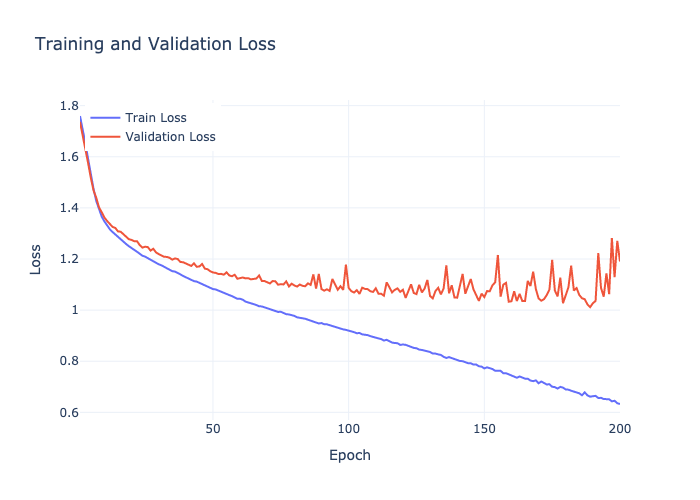
\includegraphics[width=\textwidth]{images/mlp-training-validation-loss-batch-64-lr-0.002-epochs-200-hidden-200-dropout-0.01-l2-0.0-layers-2-act-relu-opt-sgd-mom-0.0.png}
        \caption{Dropout = $0.01$}
    \end{subfigure}
    \begin{subfigure}{0.32\textwidth}
        \centering
        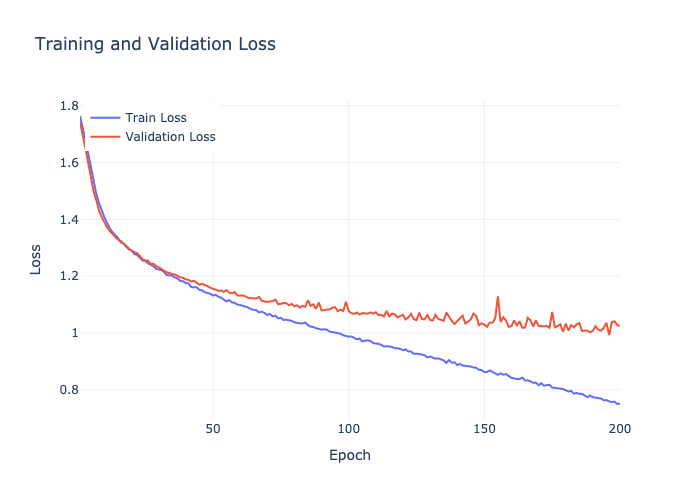
\includegraphics[width=\textwidth]{images/mlp-training-validation-loss-batch-64-lr-0.002-epochs-200-hidden-200-dropout-0.25-l2-0.0-layers-2-act-relu-opt-sgd-mom-0.0.png}
        \caption{Dropout = $0.25$}
    \end{subfigure}
    \begin{subfigure}{0.32\textwidth}
        \centering
        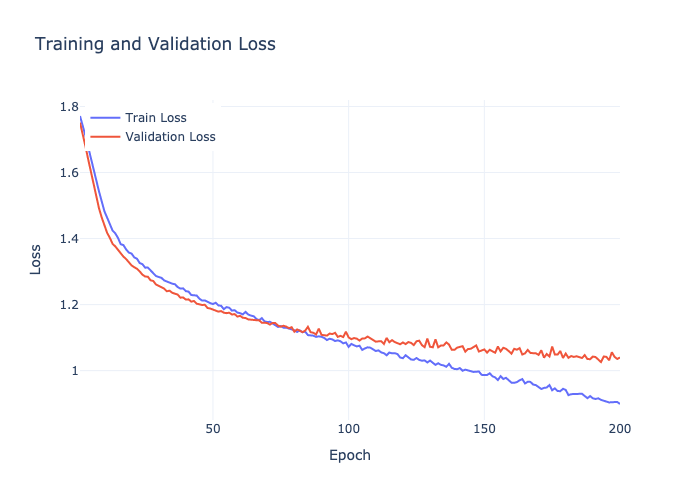
\includegraphics[width=\textwidth]{images/mlp-training-validation-loss-batch-64-lr-0.002-epochs-200-hidden-200-dropout-0.5-l2-0.0-layers-2-act-relu-opt-sgd-mom-0.0.png}
        \caption{Dropout = $0.5$}
    \end{subfigure}
    \caption{MLP: Training and Validation Loss for different Dropout values.}
    \label{fig:mlp_dropout_loss}
\end{figure}

% MLP: Validation Accuracy (Effect of Dropout)
\subsection{MLP: Validation Accuracy (Effect of Dropout)}
\begin{figure}[htbp!]
    \centering
    \begin{subfigure}{0.32\textwidth}
        \centering
        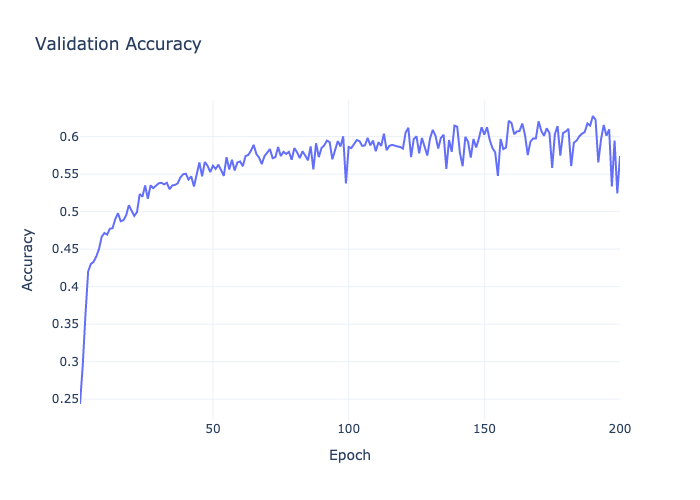
\includegraphics[width=\textwidth]{images/mlp-validation-accuracy-batch-64-lr-0.002-epochs-200-hidden-200-dropout-0.01-l2-0.0-layers-2-act-relu-opt-sgd-mom-0.0.png}
        \caption{Dropout = $0.01$}
    \end{subfigure}
    \begin{subfigure}{0.32\textwidth}
        \centering
        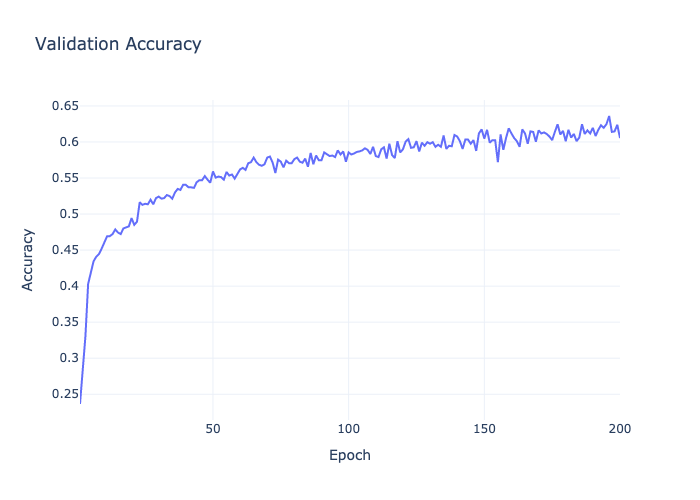
\includegraphics[width=\textwidth]{images/mlp-validation-accuracy-batch-64-lr-0.002-epochs-200-hidden-200-dropout-0.25-l2-0.0-layers-2-act-relu-opt-sgd-mom-0.0.png}
        \caption{Dropout = $0.25$}
    \end{subfigure}
    \begin{subfigure}{0.32\textwidth}
        \centering
        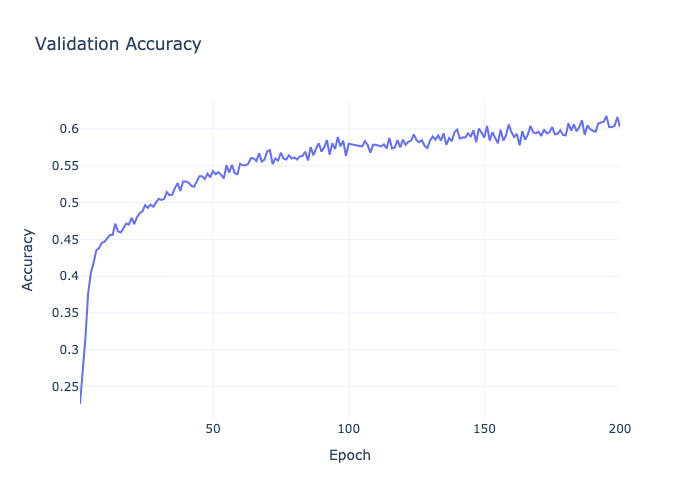
\includegraphics[width=\textwidth]{images/mlp-validation-accuracy-batch-64-lr-0.002-epochs-200-hidden-200-dropout-0.5-l2-0.0-layers-2-act-relu-opt-sgd-mom-0.0.png}
        \caption{Dropout = $0.5$}
    \end{subfigure}
    \caption{MLP: Validation Accuracy for different Dropout values.}
    \label{fig:mlp_dropout_acc}
\end{figure}

\clearpage

% MLP: Momentum Effects
\subsection{MLP: Effect of Momentum}
\begin{figure}[htbp!]
    \centering
    \begin{subfigure}{0.45\textwidth}
        \centering
        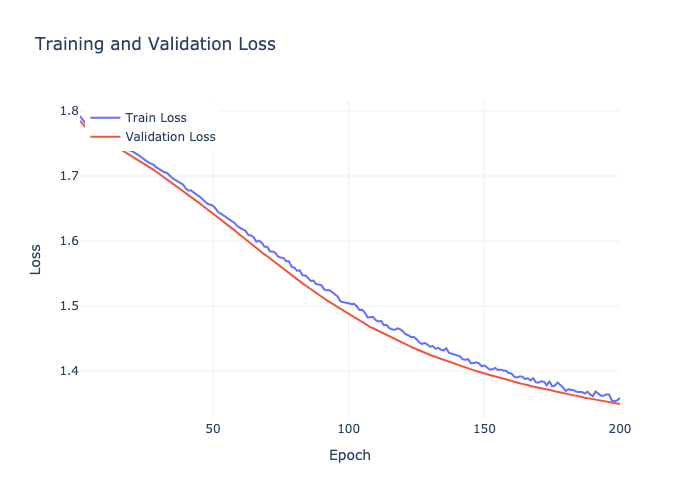
\includegraphics[width=\textwidth]{images/mlp-training-validation-loss-batch-1024-lr-0.002-epochs-200-hidden-200-dropout-0.3-l2-0.0-layers-2-act-relu-opt-sgd-mom-0.0.png}
        \caption{Momentum = $0.0$}
    \end{subfigure}
    \begin{subfigure}{0.45\textwidth}
        \centering
        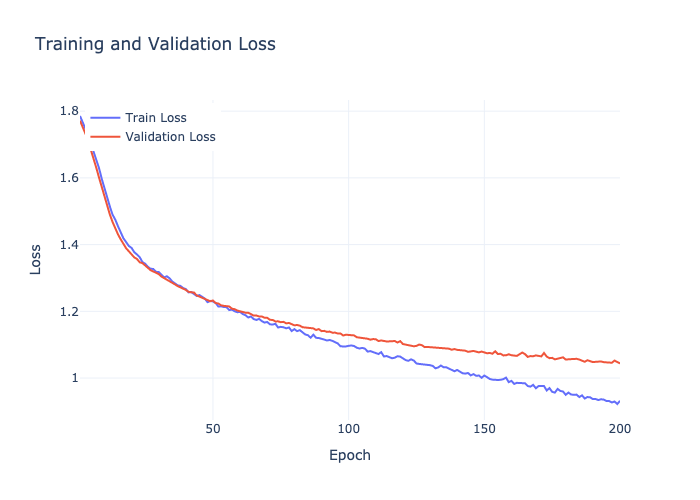
\includegraphics[width=\textwidth]{images/mlp-training-validation-loss-batch-1024-lr-0.002-epochs-200-hidden-200-dropout-0.3-l2-0.0-layers-2-act-relu-opt-sgd-mom-0.9.png}
        \caption{Momentum = $0.9$}
    \end{subfigure}
    \caption{MLP: Training and Validation Loss for different Momentum values.}
    \label{fig:mlp_momentum_loss}
\end{figure}

\begin{figure}[htbp!]
    \centering
    \begin{subfigure}{0.45\textwidth}
        \centering
        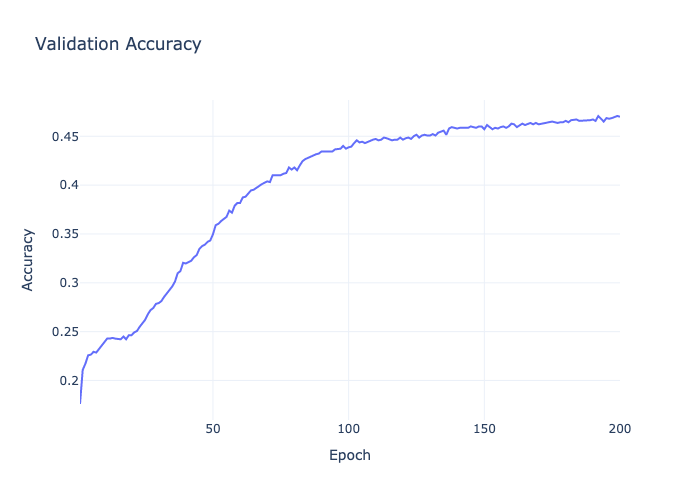
\includegraphics[width=\textwidth]{images/mlp-validation-accuracy-batch-1024-lr-0.002-epochs-200-hidden-200-dropout-0.3-l2-0.0-layers-2-act-relu-opt-sgd-mom-0.0.png}
        \caption{Momentum = $0.0$}
    \end{subfigure}
    \begin{subfigure}{0.45\textwidth}
        \centering
        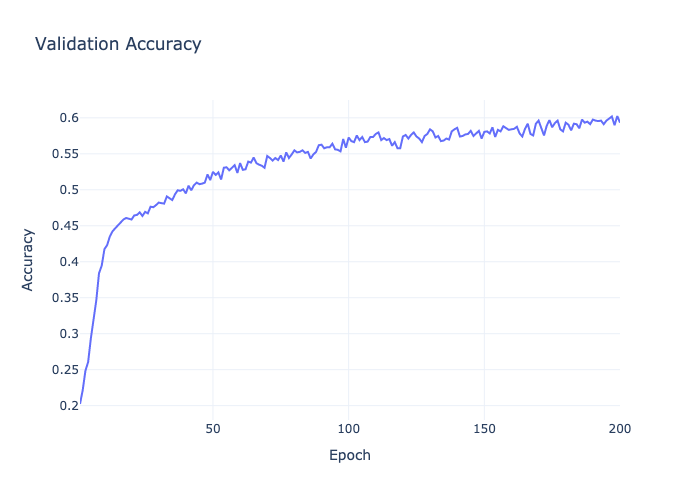
\includegraphics[width=\textwidth]{images/mlp-validation-accuracy-batch-1024-lr-0.002-epochs-200-hidden-200-dropout-0.3-l2-0.0-layers-2-act-relu-opt-sgd-mom-0.9.png}
        \caption{Momentum = $0.9$}
    \end{subfigure}
    \caption{MLP: Validation Accuracy for different Momentum values.}
    \label{fig:mlp_momentum_acc}
\end{figure}


